\documentclass[a4paper, 12pt, oneside]{extarticle}
%-shell-escape % якщо використовуєте minted
\input{$HOME/Templates/lpnu_doc_templates/settings/preamble.tex}
% якщо домахуються дуже за Times New Roman, то
% використовуєте xelatex і цей файл:
\input{$HOME/Templates/lpnu_doc_templates/settings/font_styles.tex}

\newcommand\Variant{4}
\newcommand\Date{13.03.\the\year}
\newcommand\Discipline{Алгоритмізація та програмування, частина 2}
\newcommand\Instructor{Кулешник Я. Ф.}

\newcommand\Lab{лабораторної роботи}
\newcommand\Pract{практичної роботи}
\newcommand\Work{\Lab~\No2}
\newcommand\Topic{Машина Тюрінга}

\begin{document}
\Margins

\input{$HOME/Templates/lpnu_doc_templates/parts/header.tex}

Вивчення формального визначення поняття алгоритму,
пов’язаного із введеною Аланом Тьюрінґом спеціальної математичної
конструкції (машина Тюрінга) і постулювання тези про еквівалентність

\section*{Індивідуальне завдання}

Задано масив з дужок, що відкриваються і закриваються. Побудувати
машину Тюрінґа, яка видаляла б пари взаємних дужок. Наприклад,
початковий стан: « ) ( ( ) ( ( ) », кінцевий стан: « ) . . . ( ( . ».

\section*{Етапи розв'язку}

\subsection*{Код програми}

\begin{figure}[h]
	\centering
	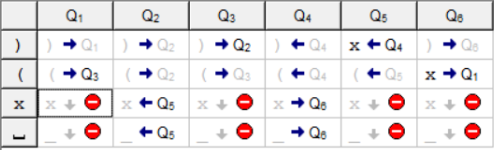
\includegraphics[width=.5\textwidth]{commands.png}
	\caption{Таблиця правил переходу}
\end{figure}

\subsection*{Результат виконання програми}

\begin{figure}[h]
	\begin{subfigure}{.5\textwidth}
		\centering
		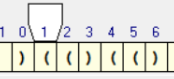
\includegraphics[width=.5\textwidth]{in.png}
		\subcaption{Вхідні дані}
	\end{subfigure}
	\hfill
	\begin{subfigure}{.5\textwidth}
		\centering
		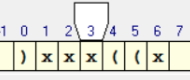
\includegraphics[width=.55\textwidth]{out.png}
		\subcaption{Вихідні дані}
	\end{subfigure}
	\caption{Демонстрація роботи програми}
\end{figure}

\section*{Висновок}

Ця лабораторна робота познайомила мене з написанням програм для машини Тюріна.
Хочу зазначити, що ця машина складніша за машину Поста, але ця складність
спрощує реалізацію алгоритмів.

\section*{Відповіді на контрольні запитання}
\begin{itemize}

	\question З чого складається машина Тюрінга? Які дії вона виконує?

\answer До складу машини Тюрінга входить необмежена в обидві сторони
стрічка (можливі машини Тюрінга, які мають кілька нескінченних стрічок),
розділена на комірки, і керуючий пристрій (також називається головкою
запису-читання (ГЗЧ)), що здатен перебувати в одному із множини станів.
Число можливих станів керуючого пристрою скінченне і точно задано.

ГЗЧ може рухатися по стрічці та записувати в комірки символи алфавіту
згідно з програмою.

	\question За допомогою чого описують машину Тюрінга? Наведіть приклади
	\answer Для опису машини Тюрінга використовуються наступні елементи:

		\begin{itemize}
			\item Стрічка - це послідовність символів з певного алфавіту. Символи на стрічці можуть бути змінені керуючим пристроєм машини Тюрінга.

			\item Головка - це пристрій, що може переміщуватися по стрічці та зчитувати символи на ній. Головка може змінювати символи на стрічці та переміщуватися вліво або вправо.

			\item Стан - це стан машини, який визначає поведінку машини в конкретний момент часу. Машина Тюрінга може знаходитися в одному зі скінченного числа станів.

			\item Правила переходу - це правила, які описують, як машина Тюрінга повинна змінювати свій стан та символи на стрічці під час роботи. Правила переходу зазвичай описуються у вигляді таблиці або діаграми.
		\end{itemize}

	\question Що називають композицією машин Тюрінга?

	\answer Композицією називають створення машини Тюрінга з сукупності машин Тюрінга.

	\question В чому полягає задача універсального алгоритму?
	\answer Задача універсального алгоритму полягає у створенні алгоритму, який може симулювати будь-який інший алгоритм, знаючи його опис у вигляді коду. Іншими словами, універсальний алгоритм може виконувати функції будь-якого іншого алгоритму, який може бути описаний у вигляді машини Тюрінга або в будь-якій іншій формі.

	\question Що таке універсальна машина Тюрінґа?

\answer Універсальна машина Тюрінга(УМТ) --- це така машина Тюрінга(МТ)
яка може замінити собою будь-яку машину Тюрінга. Вона зберігає на стрічці
не лише дані для опрацювання, але й програми для машини тюрінга, які вона запускає згідно зі своєю таблицею.

\end{itemize}

\end{document}
